\providecommand{\relativeRoot}{../..}
\documentclass[\relativeRoot/main.tex]{subfiles}
\graphicspath{
    {\subfix{./figures/}}
}

\begin{document}

\chapter{Introduction}
\label{chap:intro}

\begin{figure}
    \centering
    \begin{tikzpicture}[line width=3pt, line cap=round]
        \node [above right, inner sep=0] (image) at (0,0) {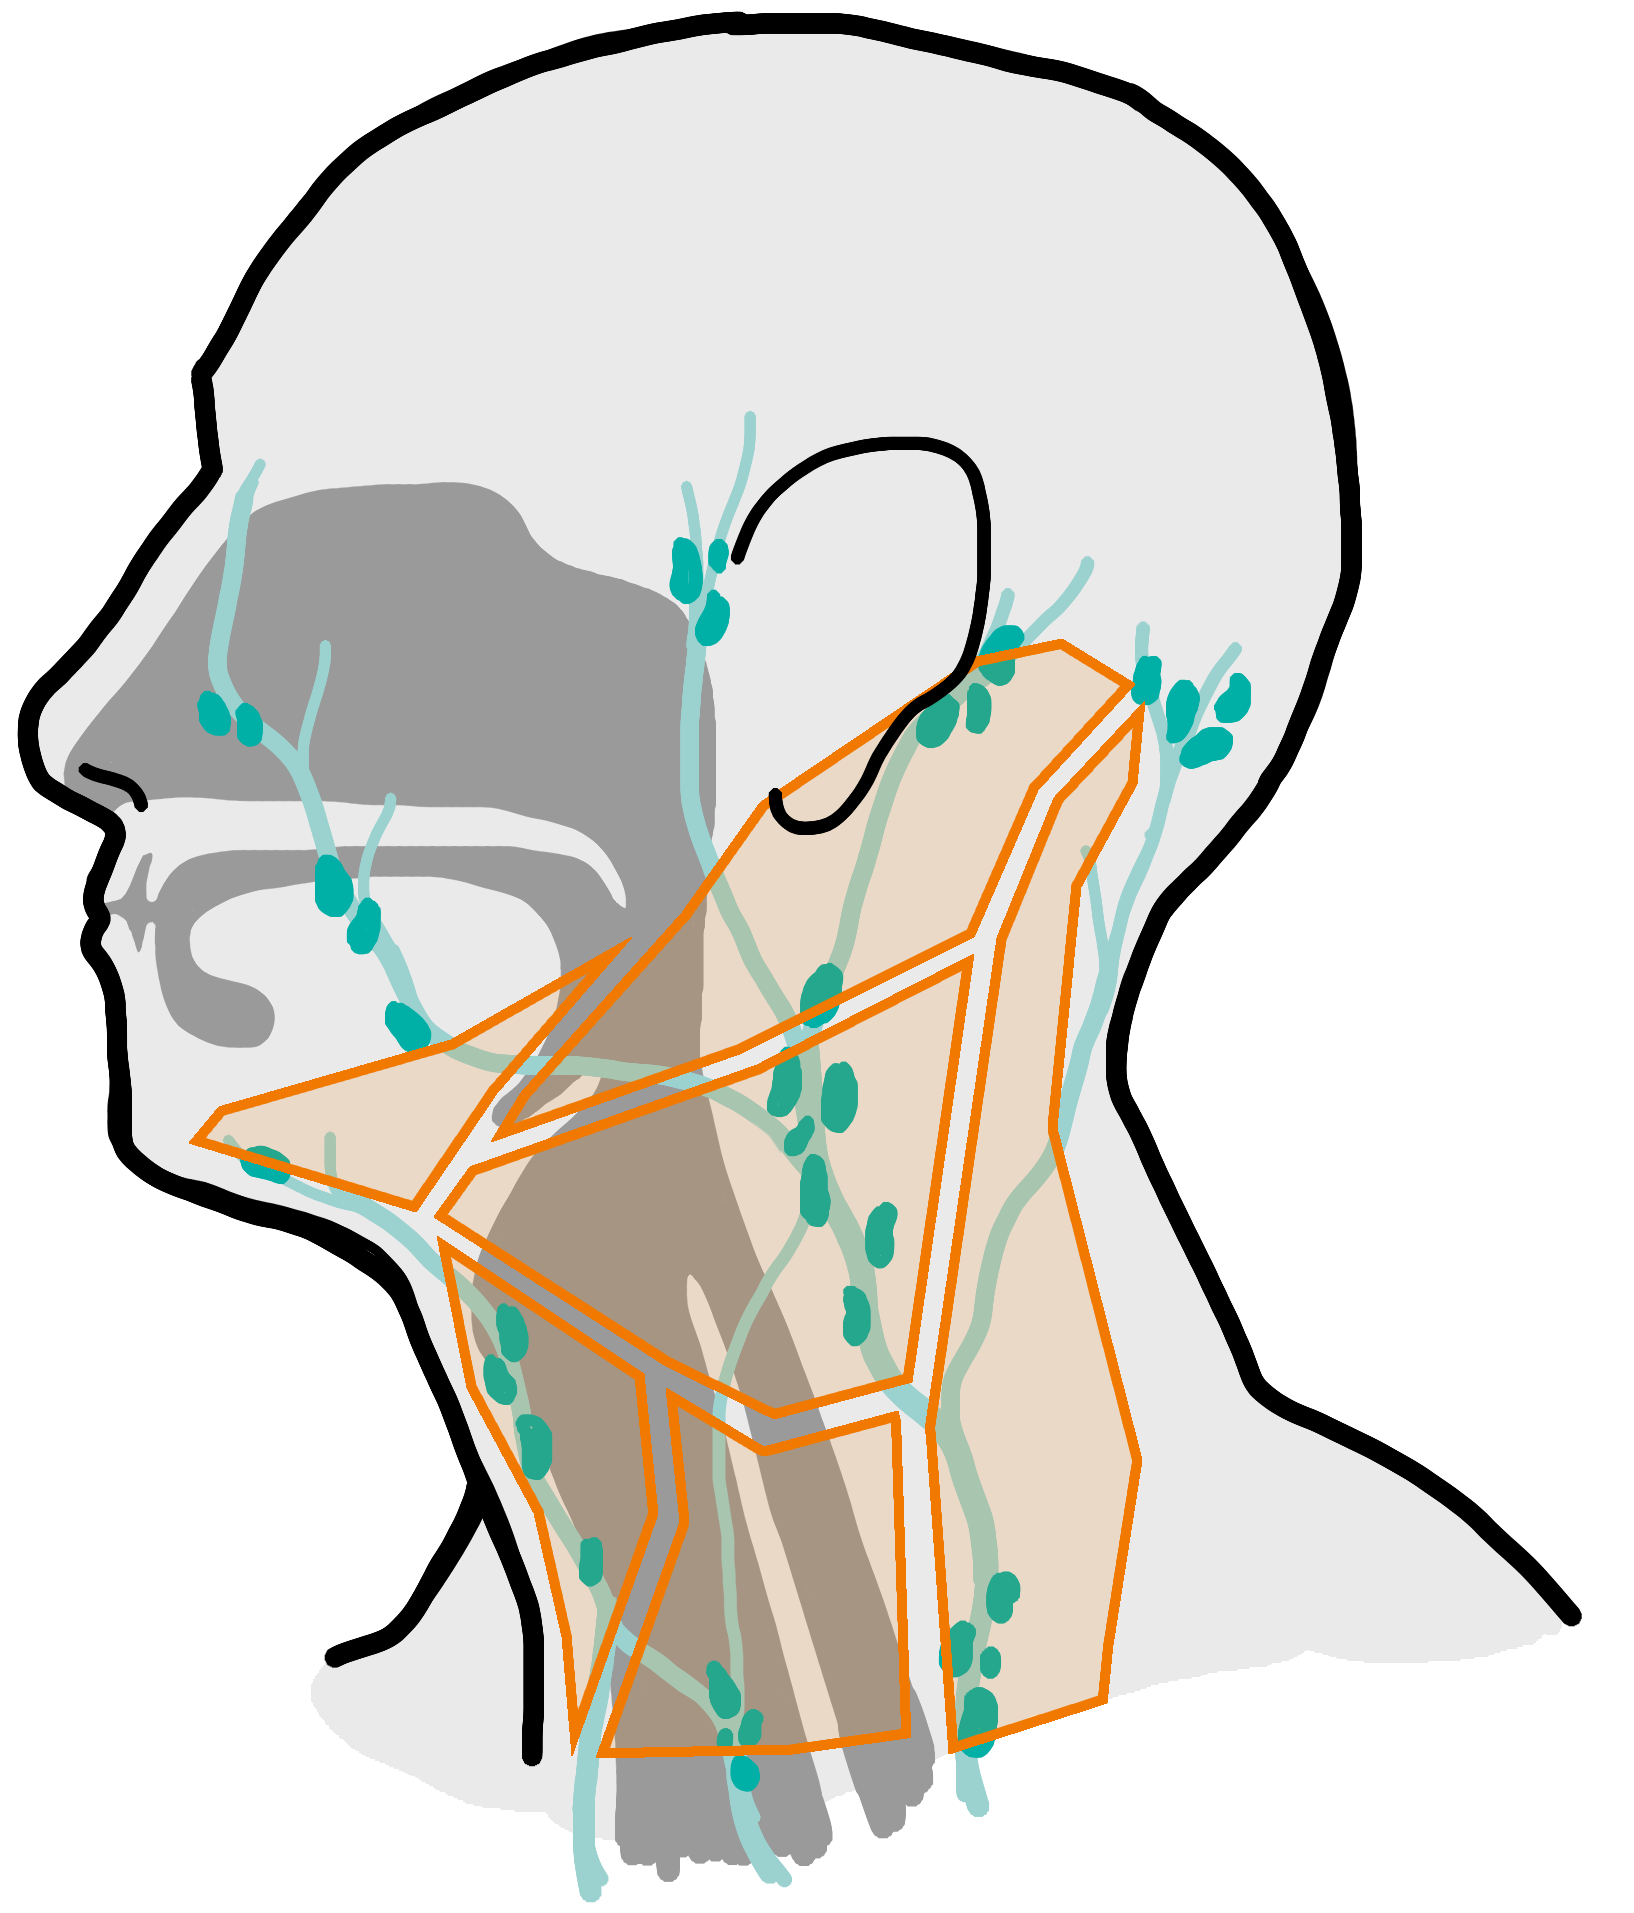
\includegraphics[width=\textwidth]{figures/head_and_neck.png}};

        % Create scope with normalized axes
        \begin{scope}[
            x={($0.1*(image.south east)$)},
            y={($0.1*(image.north west)$)}]
        
        % Grid
            \draw[lightgray,step=1,line width=1pt] (image.south west) grid (image.north east);
        
        % Axes' labels
            \foreach \x in {0,1,...,10} { \node [below] at (\x,0) {\x}; }
            \foreach \y in {0,1,...,10} { \node [left] at (0,\y) {\y};}
        
        % Labels
            \draw [uszorange] (7.5,7.5) -- (6.7,6.5);
            \node[circle,white,fill=uszorange,minimum size=30] at (7.5,7.5){II};

            \draw [uszorange] (5.81,4.5) -- (7.5,4.5);
            \node[circle,white,fill=uszorange,minimum size=30] at (7.5,4.5){III};

            \draw [uszorange] (6.92,2.4) -- (8.5,3);
            \node[circle,white,fill=uszorange,minimum size=30] at (8.5,3){V};

            \draw [uszorange] (1.8,3.9) -- (1,3);
            \node[circle,white,fill=uszorange,minimum size=30] at (1,3){I};

            \draw [uszorange] (3.2,2.3) -- (2,2);
            \node[circle,white,fill=uszorange,minimum size=30] at (2,2){VI};

            \draw [uszorange] (3.75,0.88) -- (2.5,0);
            \node[circle,white,fill=uszorange,minimum size=30] at (2.5,0){IV};

            \draw [Straight Barb-,uszblue] (2.7,6.5) -- (0,7.5) node[above]{nasal cavity};
        \end{scope}
    \end{tikzpicture}
\end{figure}

% \subfile{lymph_system}

\end{document}
